% Oct 2014
% Autor: Mandy Vogel
% session2

\documentclass[xcolor={table},c]{beamer}
%\usetheme[backgroundimagefile=mathe]{diepen}
\usetheme{Frankfurt}
% \useoutertheme{miniframes}

%\setbeamerfont{block title}{size=\small,series=\bfseries}
%\setbeamerfont{block body}{size=\footnotesize}

% \usecolortheme{beetle}

%\usepackage{handoutWithNotes}
%\pgfpagesuselayout{3 on 1 with notes}[a4paper,border shrink=5mm]

\usepackage{hyperref}
\usepackage{amssymb}


\begin{document}
\title{Second Session}   
%% \author{Toralf Kirsten \\ Mandy Vogel} 
\date{\today}

\AtBeginSection{
  \begin{frame}<beamer>{Table of Contents}
    \tableofcontents[currentsection]
  \end{frame}}

\begin{frame}
\titlepage
\end{frame}

\begin{frame}{Table of Contents}
\frametitle{Table of Contents}\tableofcontents
\end{frame}

\section{Getting Familiar}
\subsection{Working with R}
\begin{frame}\frametitle{Last time... }
  \begin{itemize}
    \item there is something called \textit{working directory} telling R where on the computer it is supposed to search for file resp. save files (via the menu, \texttt{setwd(), getwd()})
    \item there are numbers, characters and logical values (TRUE, FALSE)
    \item there is the \texttt{c()} function to create vectors
    \item there are data frames which are the R object most similar to data tables known from SPSS and Excel
    \item missing values are coded as \texttt{NA}
    \item with the \texttt{\$} I can access columns of such a \textit{data frame} 
    \item there are indices (numbers, characters, logical values)
    \item everything can be assigned to a variable
  \end{itemize}
\end{frame}

\begin{frame}\frametitle{Learned last time... $\checkmark$}
  \begin{itemize}
    \item ... and using the tab key!!!!
   \end{itemize}
\end{frame}


\section{Functions}
\subsection{Functions}
\begin{frame}\frametitle{Functions}
  \begin{itemize}
    \item we've seen them already, we've used them already
    \item they are everywhere, they do all the work
   \end{itemize}
\begin{center}
\LARGE{FUNCTIONS}
\end{center}
\end{frame}

\begin{frame}[fragile]\frametitle{Functions and Arguments}
  \begin{itemize}
  \item functions are just like what you remember from school
    \item most functions are in the following form: \texttt{f(argument1,argument2,...)}
   \end{itemize}
\end{frame}

\subsection{Arguments}

\begin{frame}[fragile]\frametitle{Functions and Arguments}
  \begin{itemize}
    \item the arguments are named, try
\begin{verbatim}
> log(x=64,base=4)
[1] 3
> log(base=4,x=64)
[1] 3
\end{verbatim}
   \end{itemize}
\end{frame}

\begin{frame}[fragile]\frametitle{Functions - Arguments}
  \begin{itemize}
  \item arguments also have a predefined order (which you can explore using the \texttt{?command})
  \item if you do not use names, they are used in this predefined order, try
\begin{verbatim}
> log(64,4)
[1] 3 
> log(4,64)
[1] 0.3333333
> ?log
\end{verbatim}
   \end{itemize}
\end{frame}


\begin{frame}[fragile]\frametitle{Functions - Arguments}
  \begin{itemize}
  \item arguments can be required
  \item or they can be optional
  \item they can have default values (again check \texttt{?command})
\begin{verbatim}
> log(64,4)
[1] 3 
> log(64)
[1] 4.158883
> ?log
\end{verbatim}
   \end{itemize}
\end{frame}

\section{Graphics}
\subsection{Histogram}
\begin{frame}[fragile]\frametitle{Histogram}
  \begin{itemize}
  \item a histogram is a set of contiguously drawn bars showing a frequency distribution
  \item bars are drawn for each group (interval) such that the area is proportional to the frequency in that group
  \item variable values are plotted on the horizontal (x-axis)
  \item frequencies on the vertical axis (y-axis)
  \item the r command (basic  graphics) is \texttt{hist()}
  \end{itemize}
\end{frame}

\begin{frame}[fragile]\frametitle{Histogram}
\begin{center}
\begin{verbatim}
> hist(islands)
\end{verbatim}
  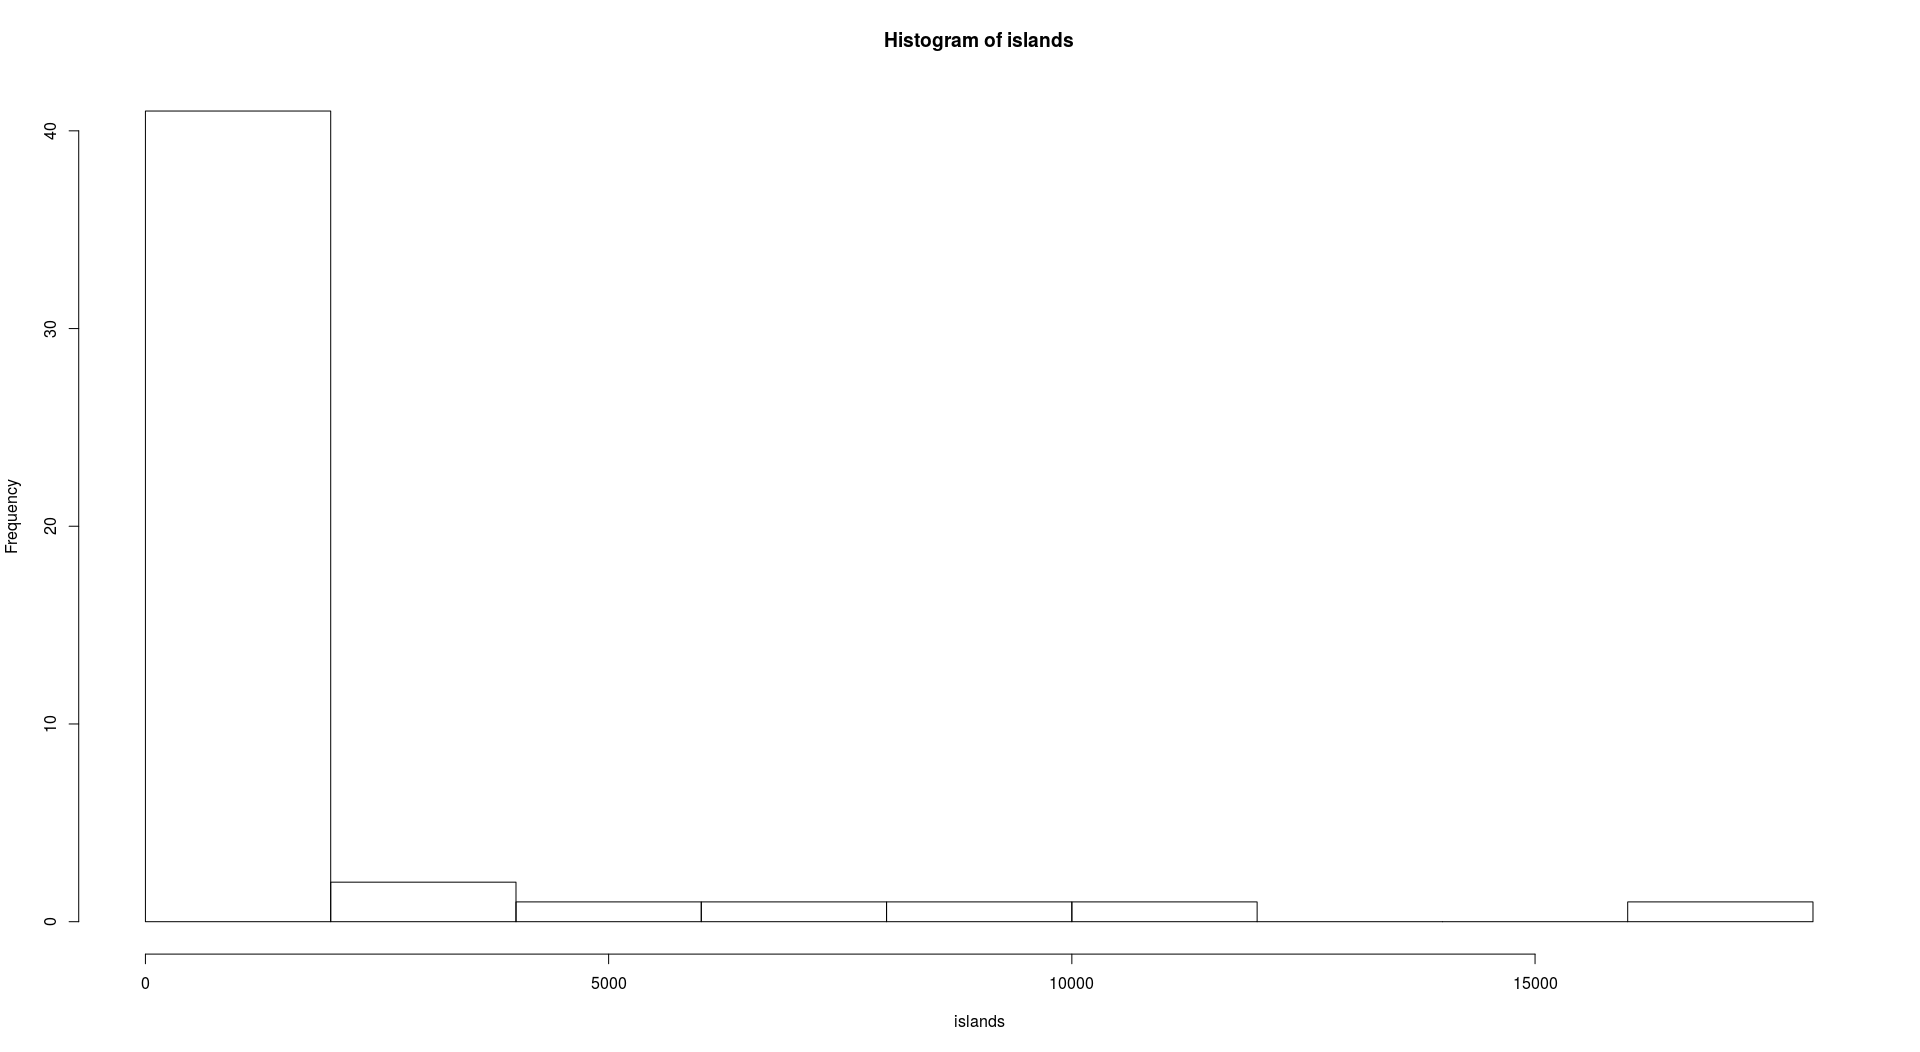
\includegraphics[width=10cm]{hist1.png}
\end{center}
\end{frame}


\begin{frame}[fragile]\frametitle{Histogram}
\begin{center}
\begin{verbatim}
> hist(islands, col = "gray", labels = TRUE)
\end{verbatim}
  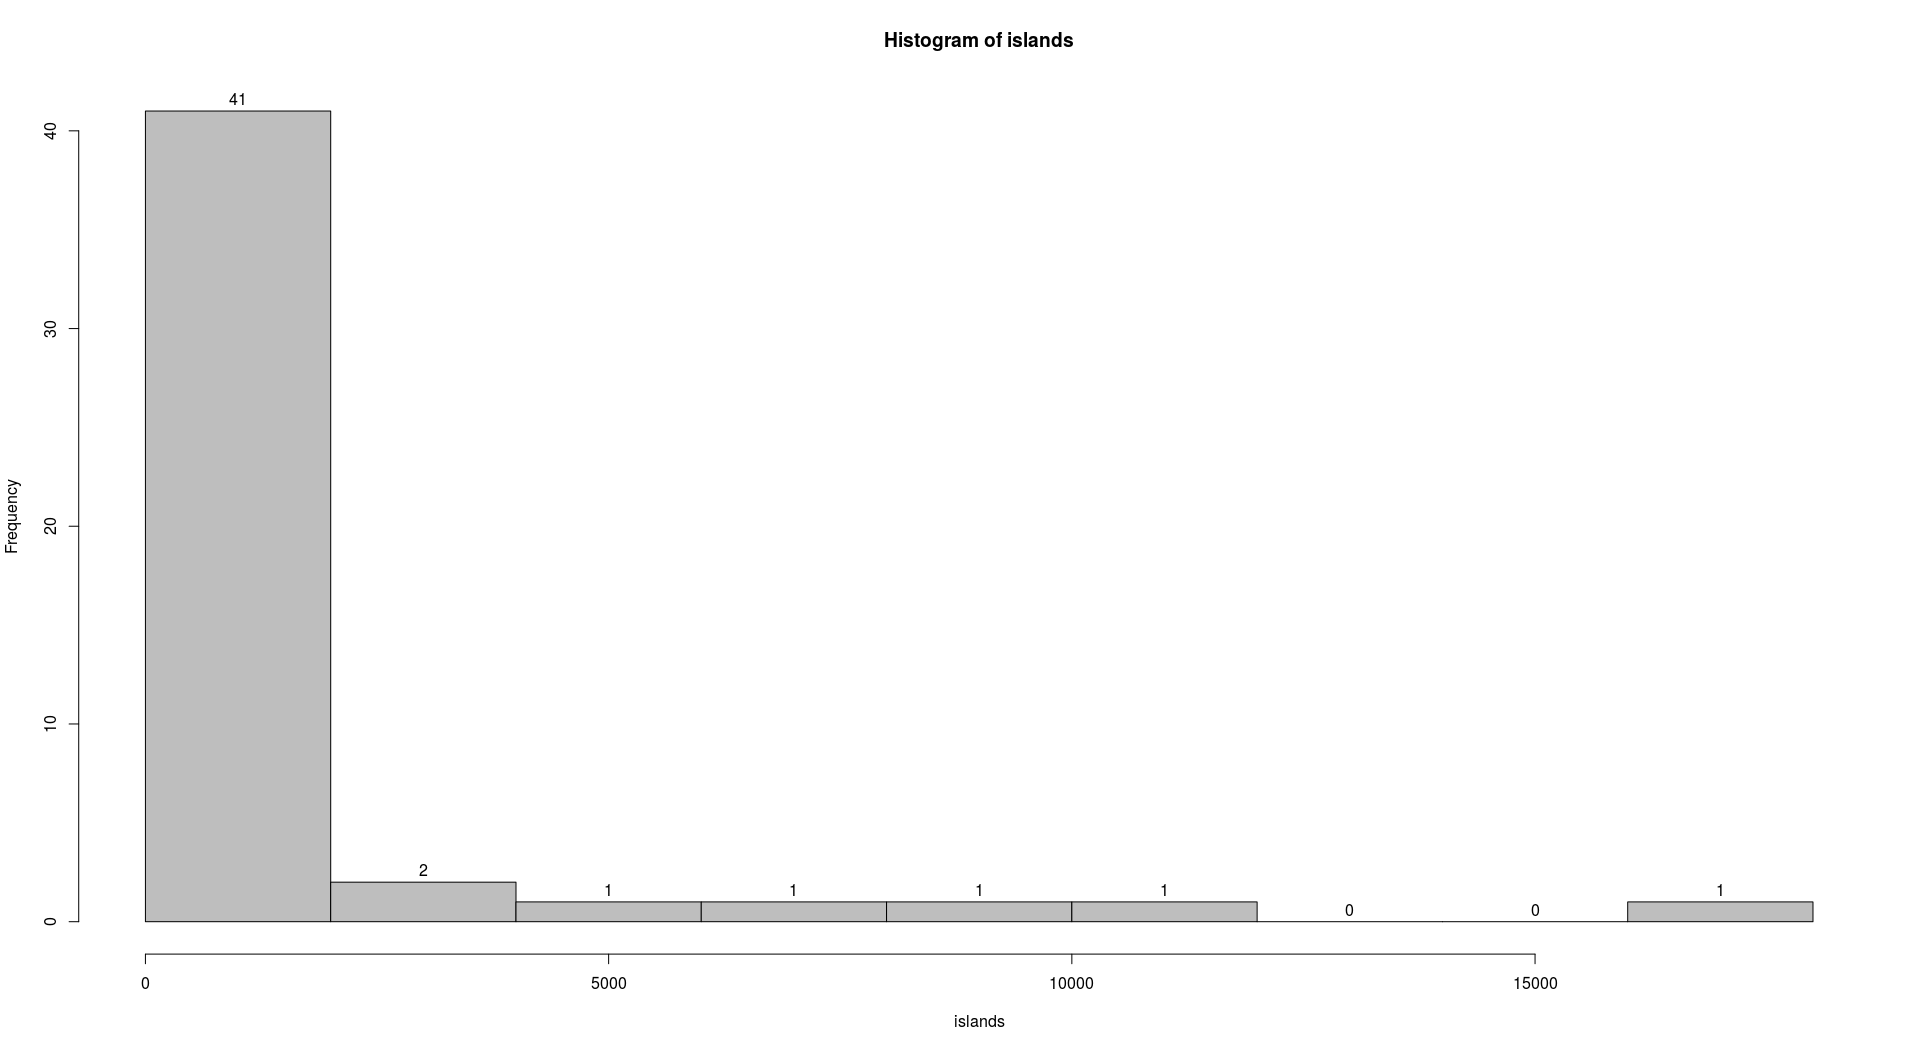
\includegraphics[width=10cm]{hist2.png}
\end{center}
\end{frame}


\begin{frame}[fragile]\frametitle{Histogram}
\begin{center}
\begin{verbatim}
> hist(sqrt(islands), breaks = 12, col = "lightblue", 
+  border = "pink")
\end{verbatim}
  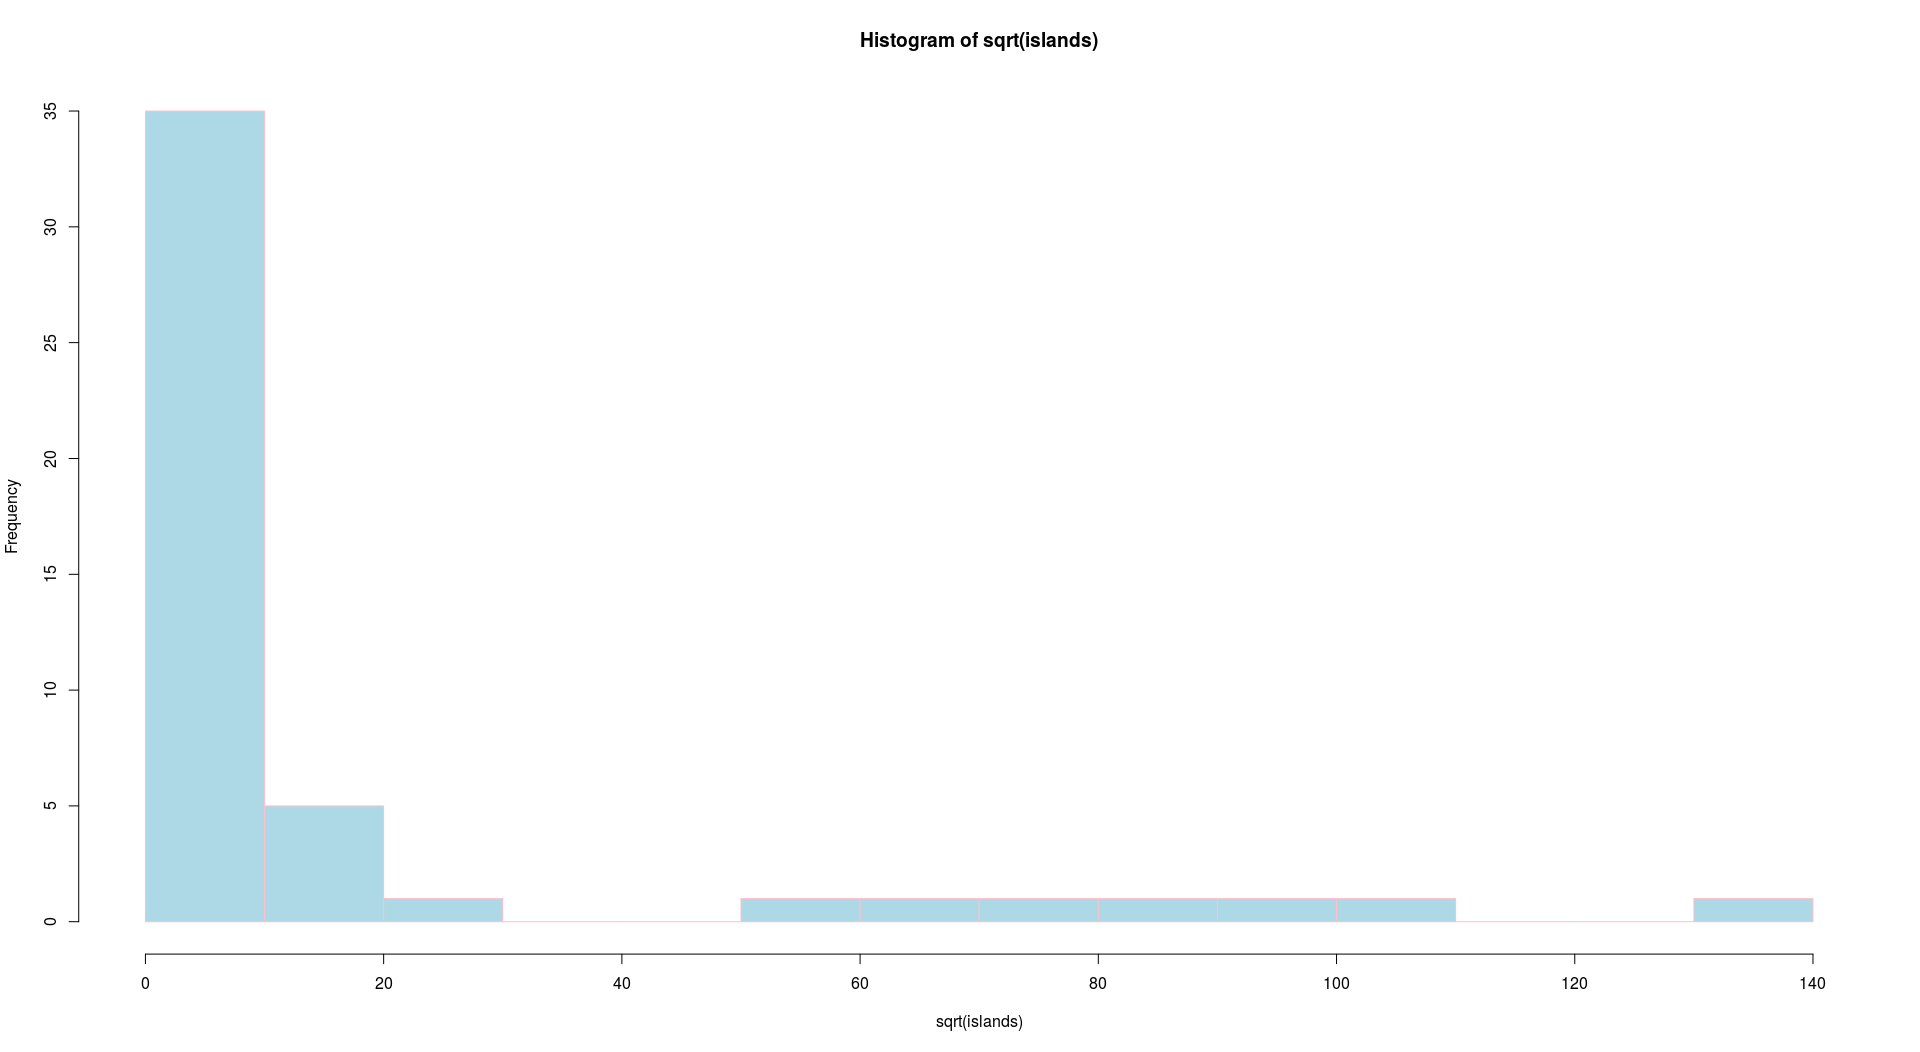
\includegraphics[width=10cm]{hist3.png}
\end{center}
\end{frame}


\begin{frame}[fragile]\frametitle{Histogram}
\begin{center}
\begin{verbatim}
r <- hist(sqrt(islands), 
+     breaks = c(4*0:5, 10*3:5, 70, 100, 140),
+     col = "blue1")
\end{verbatim}
  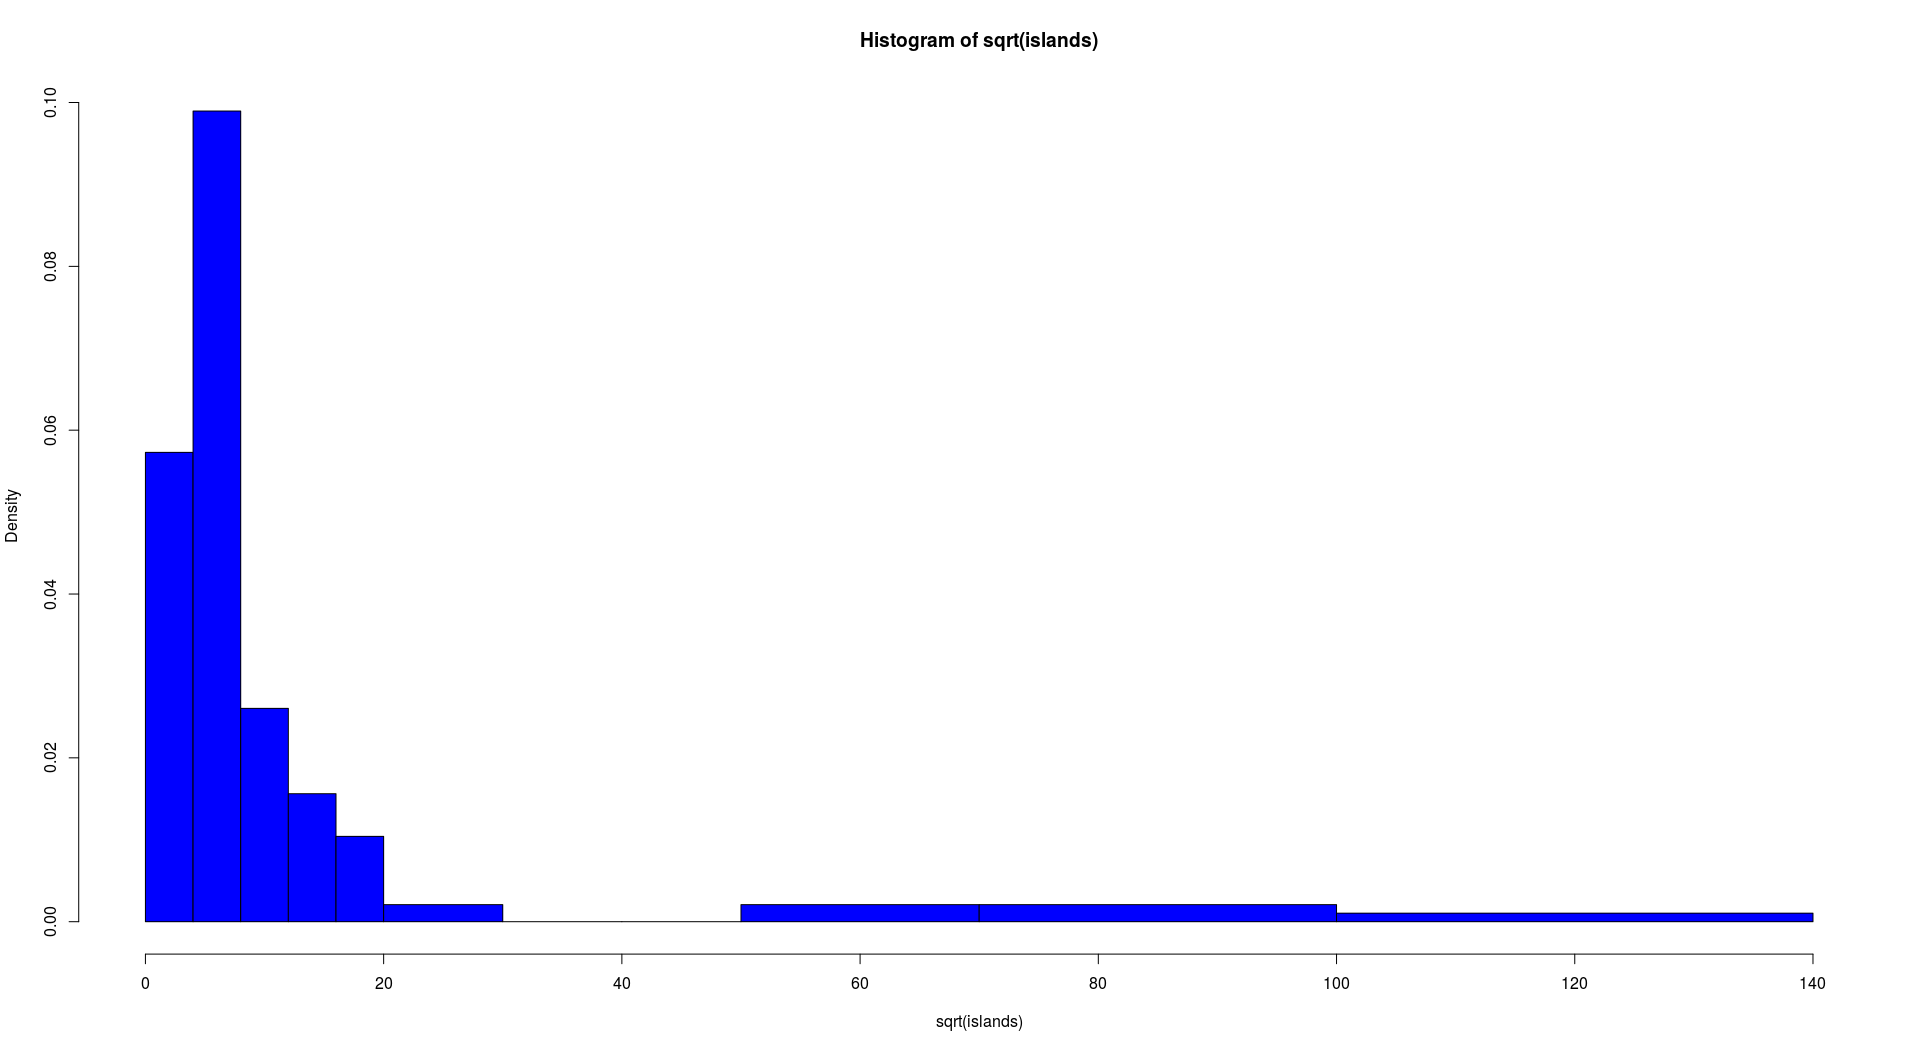
\includegraphics[width=10cm]{hist4.png}
\end{center}
\end{frame}

\begin{frame}[fragile]\frametitle{Histogram}
\begin{center}
\begin{verbatim}
> text(r$mids, r$density, r$counts, 
+  adj = c(.5, -.5), col = "blue3")
\end{verbatim}
  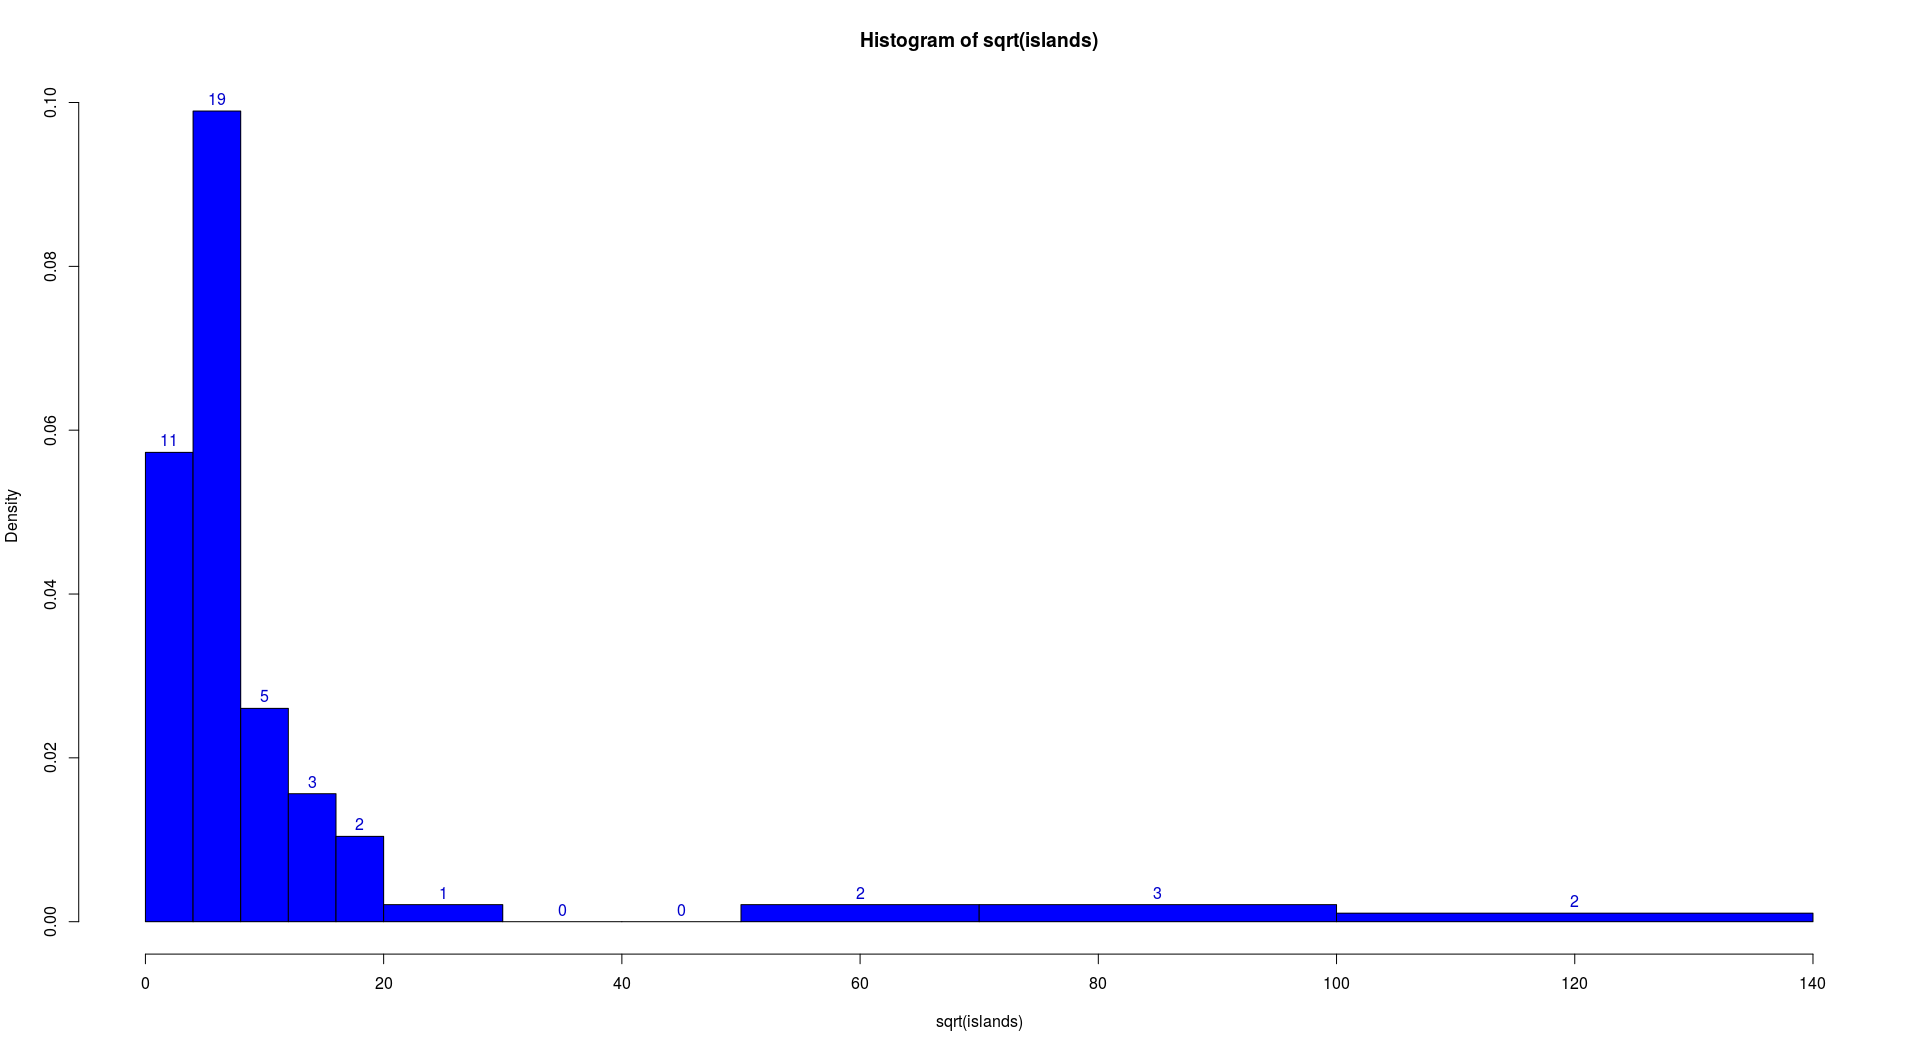
\includegraphics[width=10cm]{hist5.png}
\end{center}
\end{frame}


\begin{frame}[fragile]\frametitle{Histogram}
\begin{center}
\begin{verbatim}
> lines(r, lty = 3, border = "purple") # -> lines
\end{verbatim}
  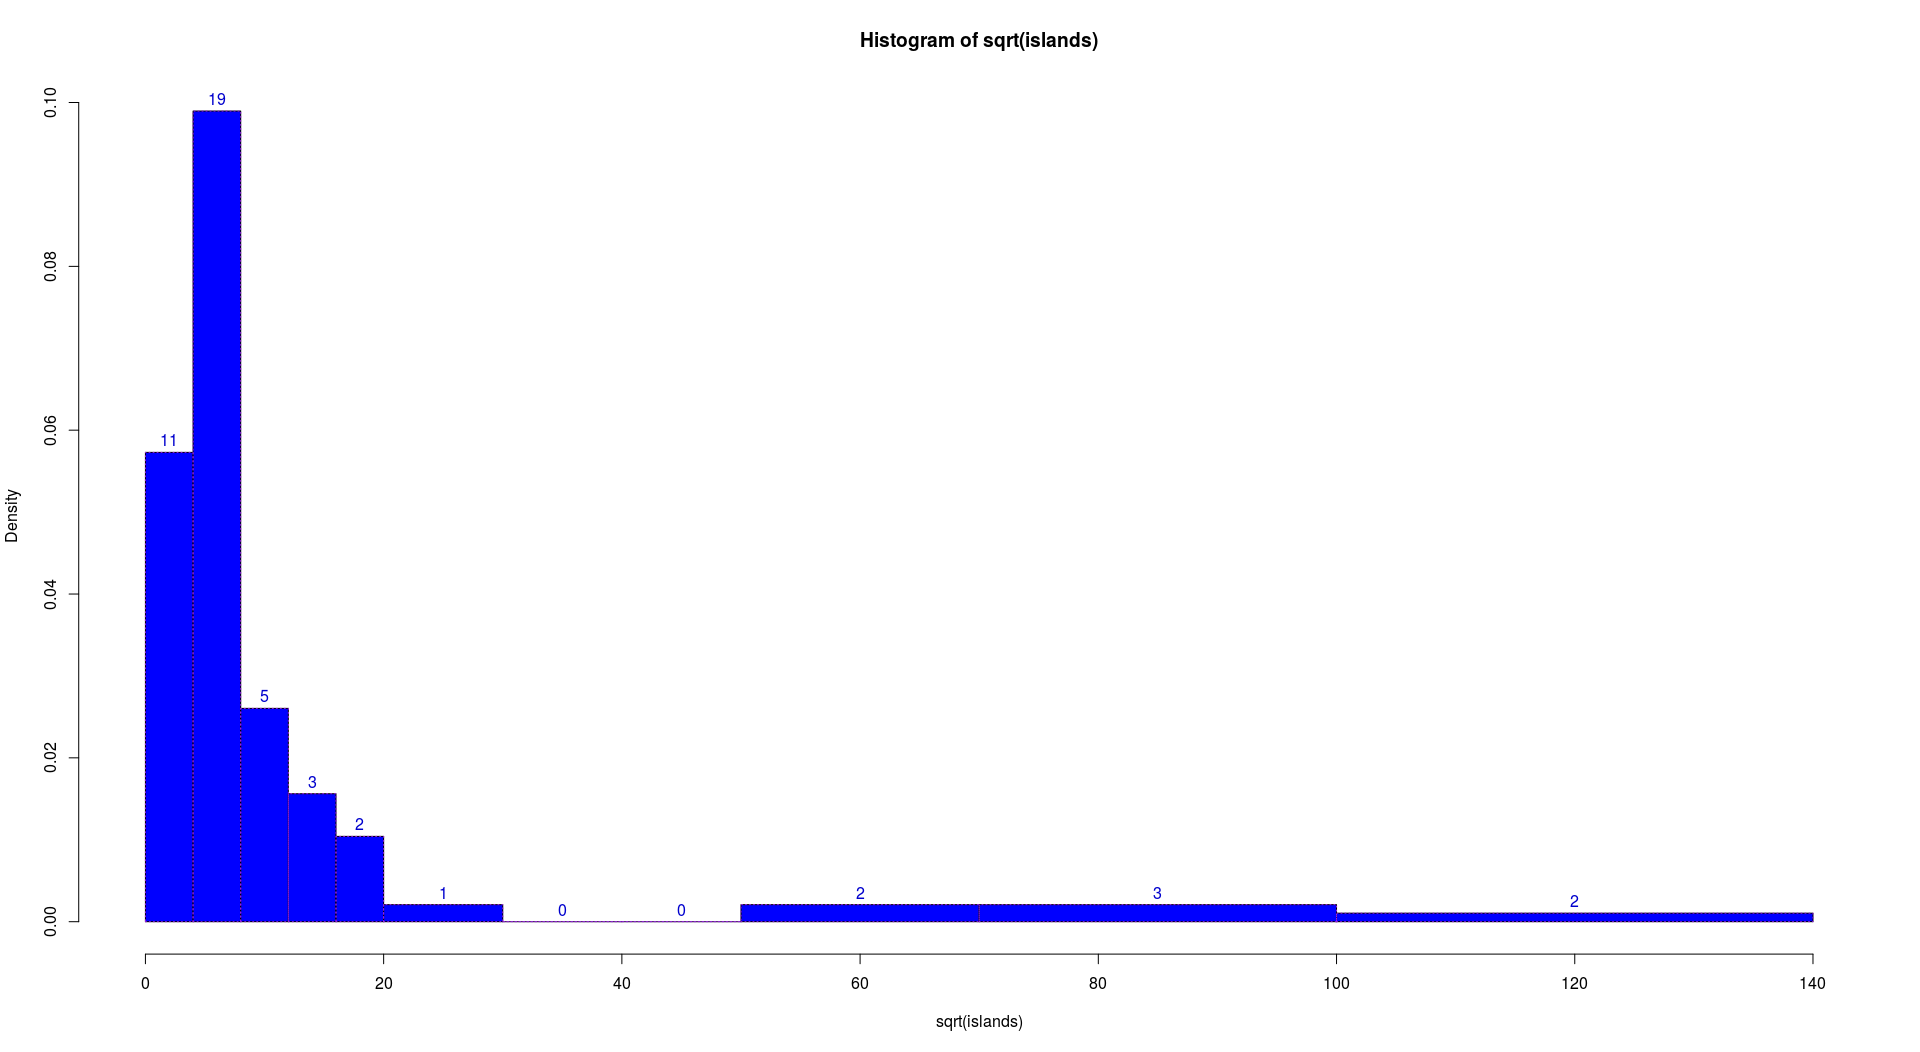
\includegraphics[width=10cm]{hist6.png}
\end{center}
\end{frame}


\begin{frame}[fragile]\frametitle{Histogram}
\begin{center}
\begin{verbatim}
> hist(islands, breaks = c(12,20,36,80,200,1000,17000), 
+  freq = TRUE, main = "WRONG histogram")
\end{verbatim}
  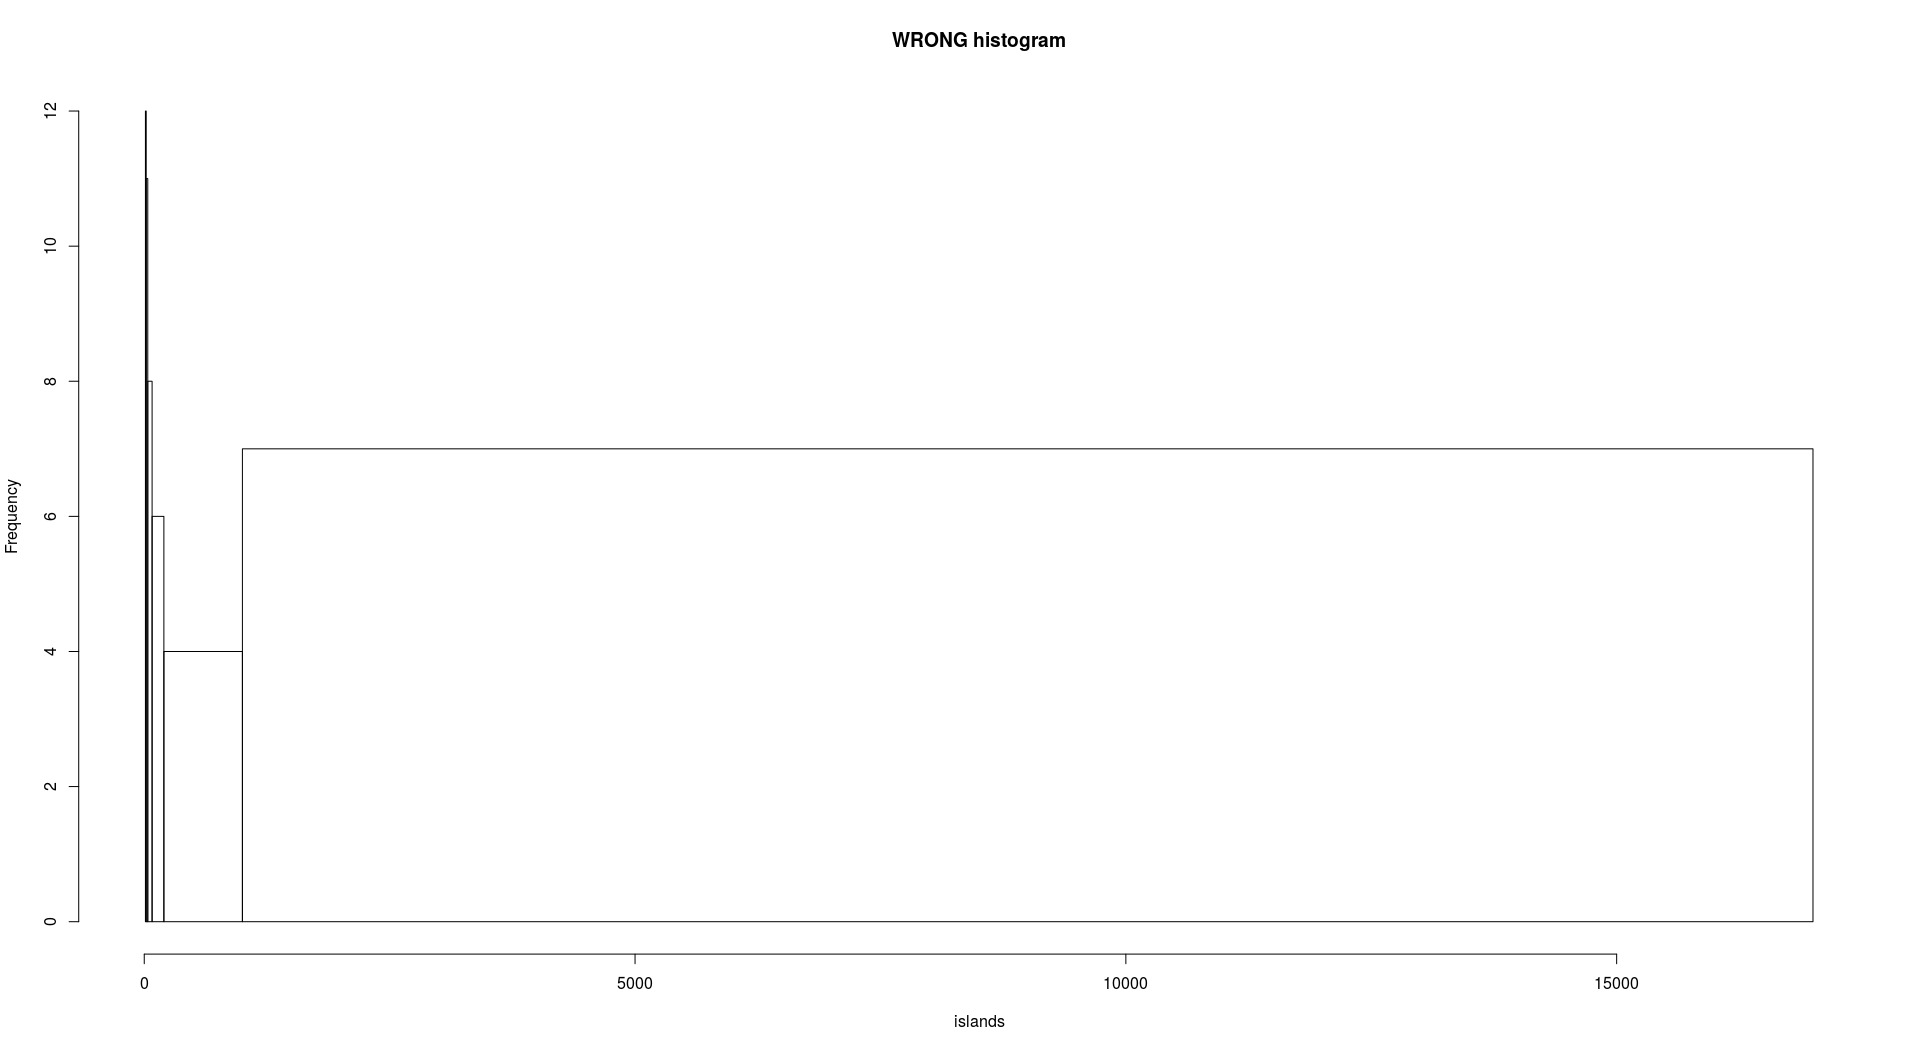
\includegraphics[width=10cm]{hist7.png}
\end{center}
\end{frame}

\begin{frame}[fragile]\frametitle{Histogram}
\begin{center}
\begin{verbatim}
> par(mfrow=c(1,2))
> set.seed(14)
> x <- rchisq(100, df = 4)
> qqplot(x, qchisq(ppoints(x), df = 4))
> abline(0, 1, col = 2, lty = 2)
> hist(x, freq = FALSE, ylim = c(0, 0.2))
> curve(dchisq(x, df = 4), col = 2, 
+  lty = 2, lwd = 2, add = TRUE)
\end{verbatim}
  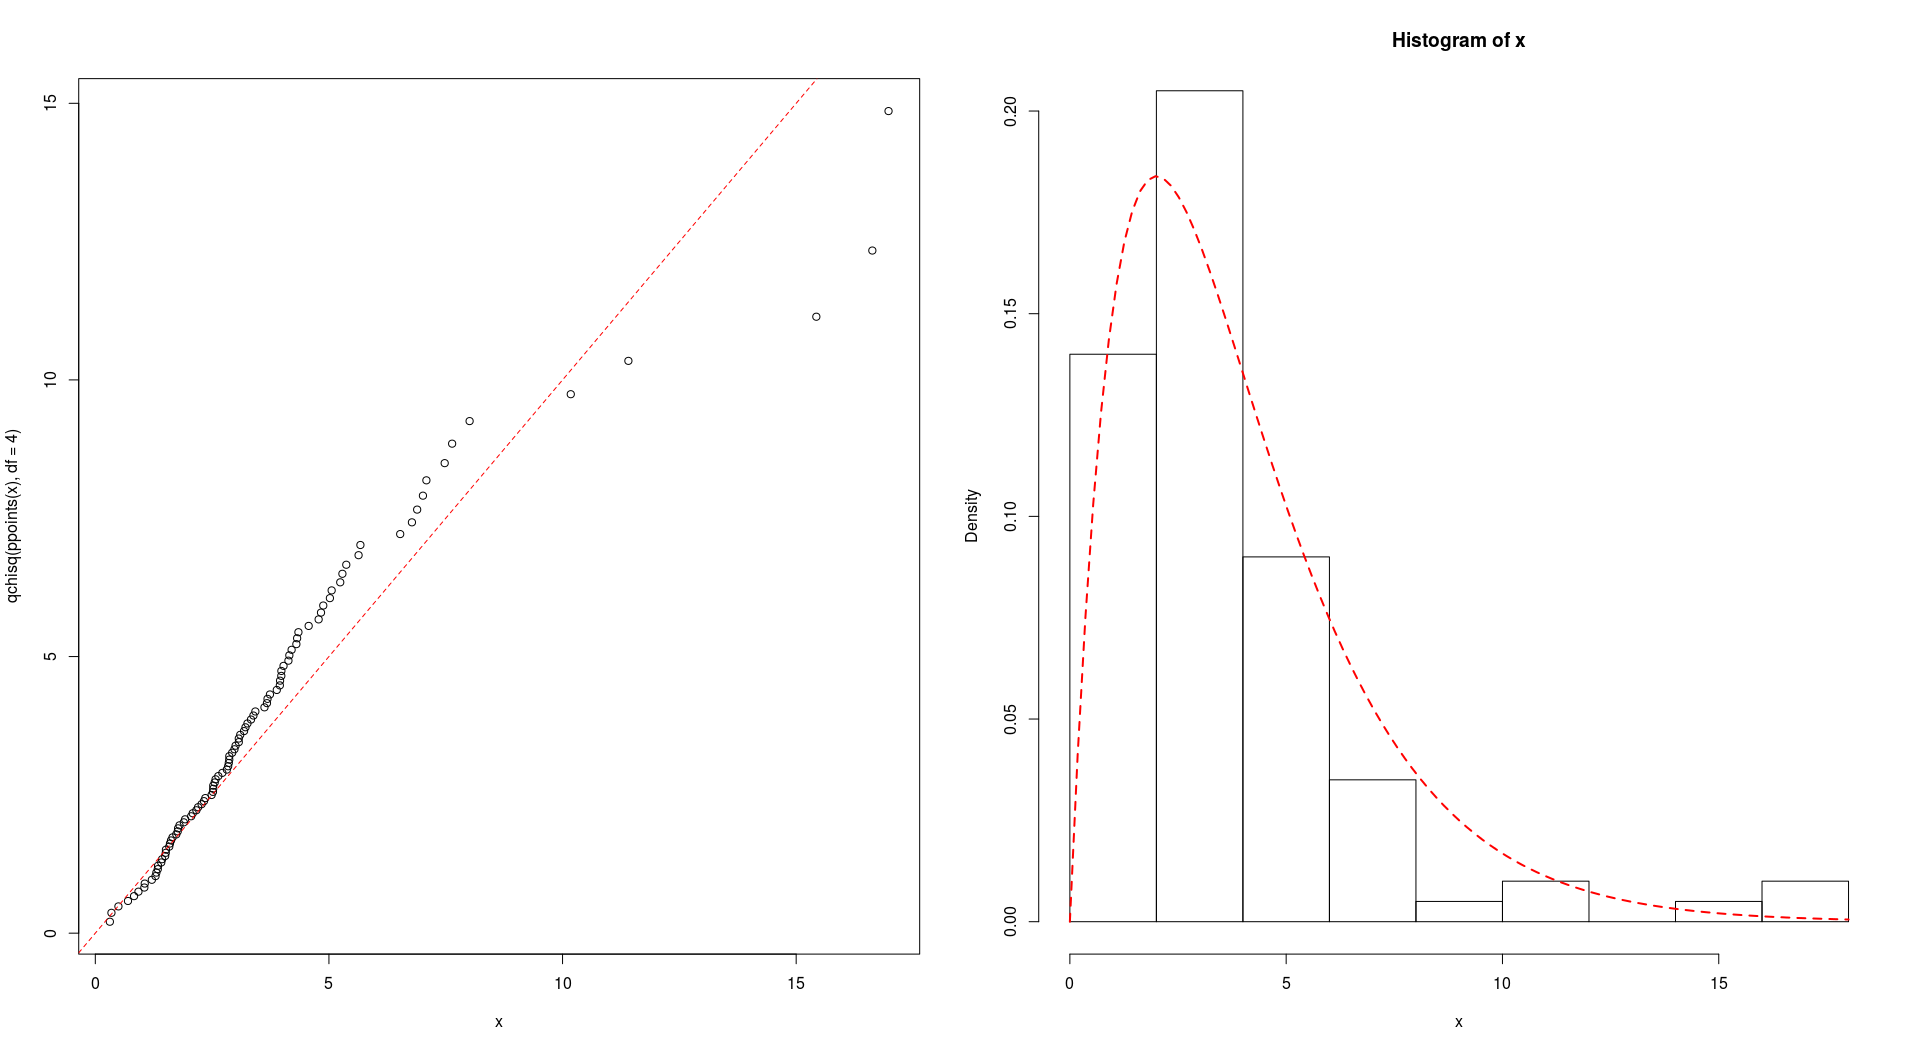
\includegraphics[width=7.5cm]{hist8.png}
\end{center}
\end{frame}

\end{document}
